\documentclass[main.tex]{subfiles}
\begin{document}
\subsection{AST Transformations}
Minipass terms are subjected to several transformations before emitting
an Overpass query. Since type information is used almost everywhere,
the term is first converted into a type-tagged term (see \cref{def:ttag})
and all transformations (including translation to Overpass) are applied
afterwards.

\cfigure{
    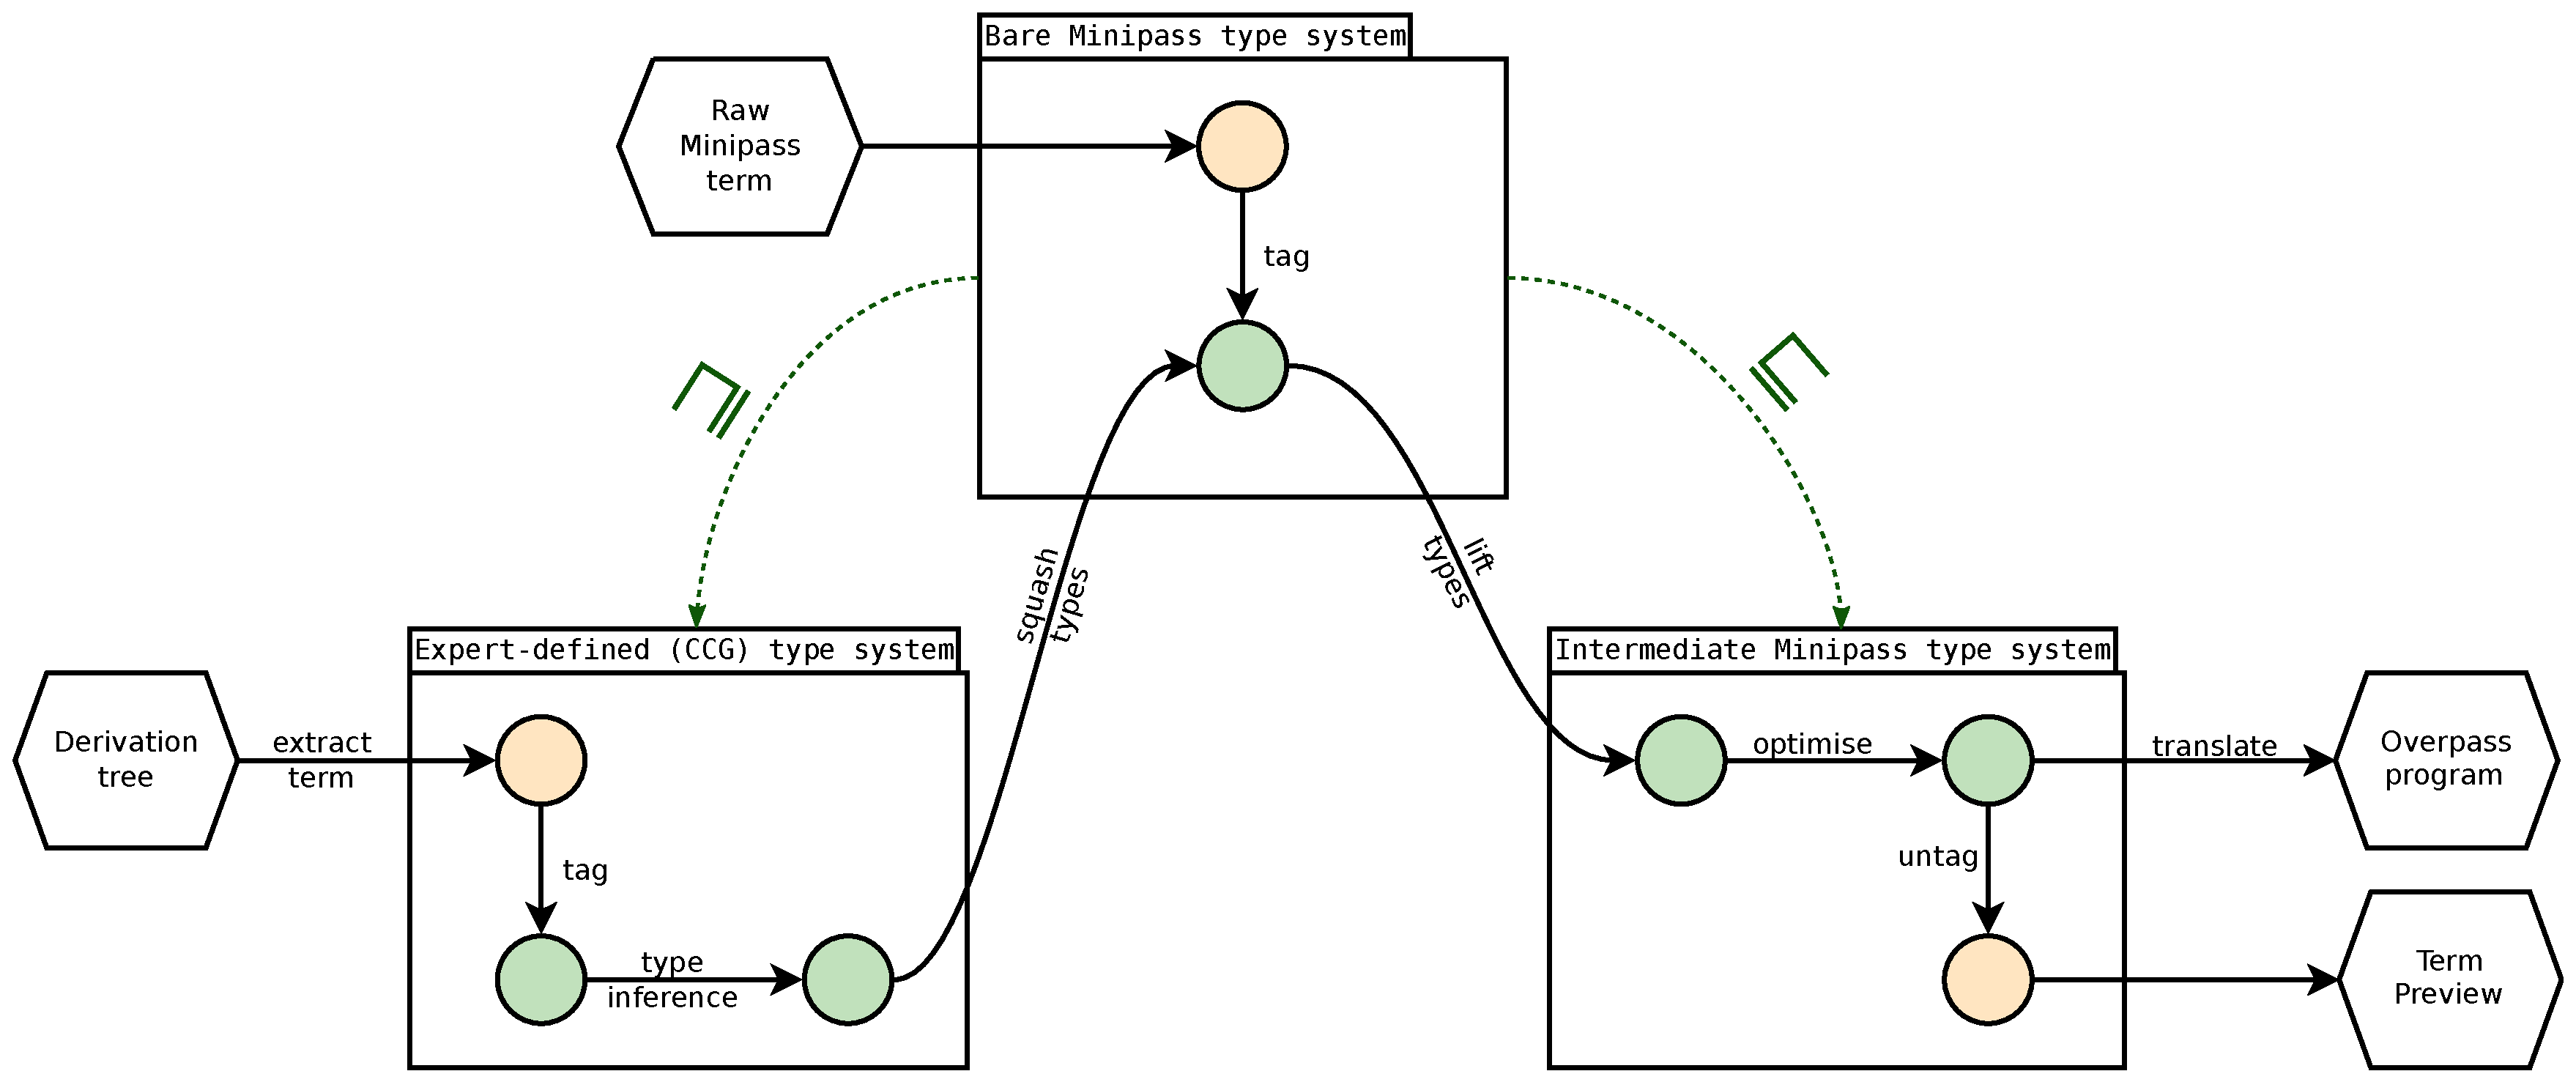
\includegraphics[width=\textwidth]{optimisation.eps}
    \caption{Illustration of the transformations a Minipass term undergoes}
    \label{fig:propagation}
}

\subsubsection{Type inference}
\label{sec:typeinf}
Minipass allows for the usage of the special type \code{*} that acts as a
wildcard type. It violates the partial order of the type lattice since it is
equivalent to all types (i.e. $\forall \sigma \in T: (\text{\code{*}} \less \sigma)
\& (\sigma \less \text{\code{*}})$).

Thus, all significant\footnote{
    Since we only work with closed terms, the only case when a type can't be
    inferred is when a bound variable is unused (for example in terms like
    \code{(\textbackslash x, y => y) 42}, where the type of \code{x} cannot be inferred).
    This, however, is harmless, because the type is unneeded anyway.
} occurances of $\code{*}$ are removed by finding the fixed point of
$\mcf{propagate}$ from \cref{def:propagation}
with the following unifier:
\[
    \sigma \unify \tau =
    \begin{cases*}
        \tau ,& $\sigma = \text{\code{*}}$ \\
        \sigma ,& $\tau = \text{\code{*}}$ \\
        \sigma ,& $\sigma = \tau$ \\
        (\sigma' \unify \tau') \tot (\sigma'' \unify \tau'') ,&
            $\sigma = (\sigma' \tot \sigma''), \tau = (\tau' \tot \tau'')$ \\
        \lnot ! ,& $\mathsf{otherwise}$ \\
    \end{cases*}
\]

Whenever the algorithm encounters a case where the unifier is not defined,
a type error is produced.

Since this unifier can only change a subtype from \code{*} to something else,
and there are a finite number of subtypes within a term, this algorithm
always terminates.

\subsubsection{Minipass query optimisation}
\label{sec:optimisation}
\fixme{write this}

\subsubsection{Translating to Overpass}
\fixme{write this}
\end{document}
